\documentclass{article}
\usepackage[utf8]{inputenc}
\usepackage[a4paper, total={6in, 9in}]{geometry}
\usepackage[francais]{babel}
\usepackage{natbib}
\usepackage{graphicx}
\usepackage{listings}
\usepackage{pdfpages}

\setlength{\parindent}{0pt}
\newcommand{\HRule}{\rule{\linewidth}{0.5mm}}

\begin{document}


\begin{titlepage}
\begin{center}


\textsc{\LARGE \'Ecole Polytechnique Fédérale de Lausanne}


\includegraphics[width=0.3\textwidth]{EPFL_logo.jpg}~\\[5cm]
% Title

{ \huge \bfseries Databases Project \\[0.4cm] }

\HRule \\[0.4cm]

{ \huge \emph{First and Second deliverable} \\[6cm] }

% Author and supervisor
\noindent
\begin{minipage}{0.4\textwidth}
\begin{center} \large
\emph{Authors:}\\
Valentine \textsc{Arrieta}\\
Morgan \textsc{Bruhin}\\
Tristan \textsc{Overney}

\end{center}
\end{minipage}%


\vfill

% Bottom of the page
{\large \today}

\end{center}
\end{titlepage}

\section{ER model}
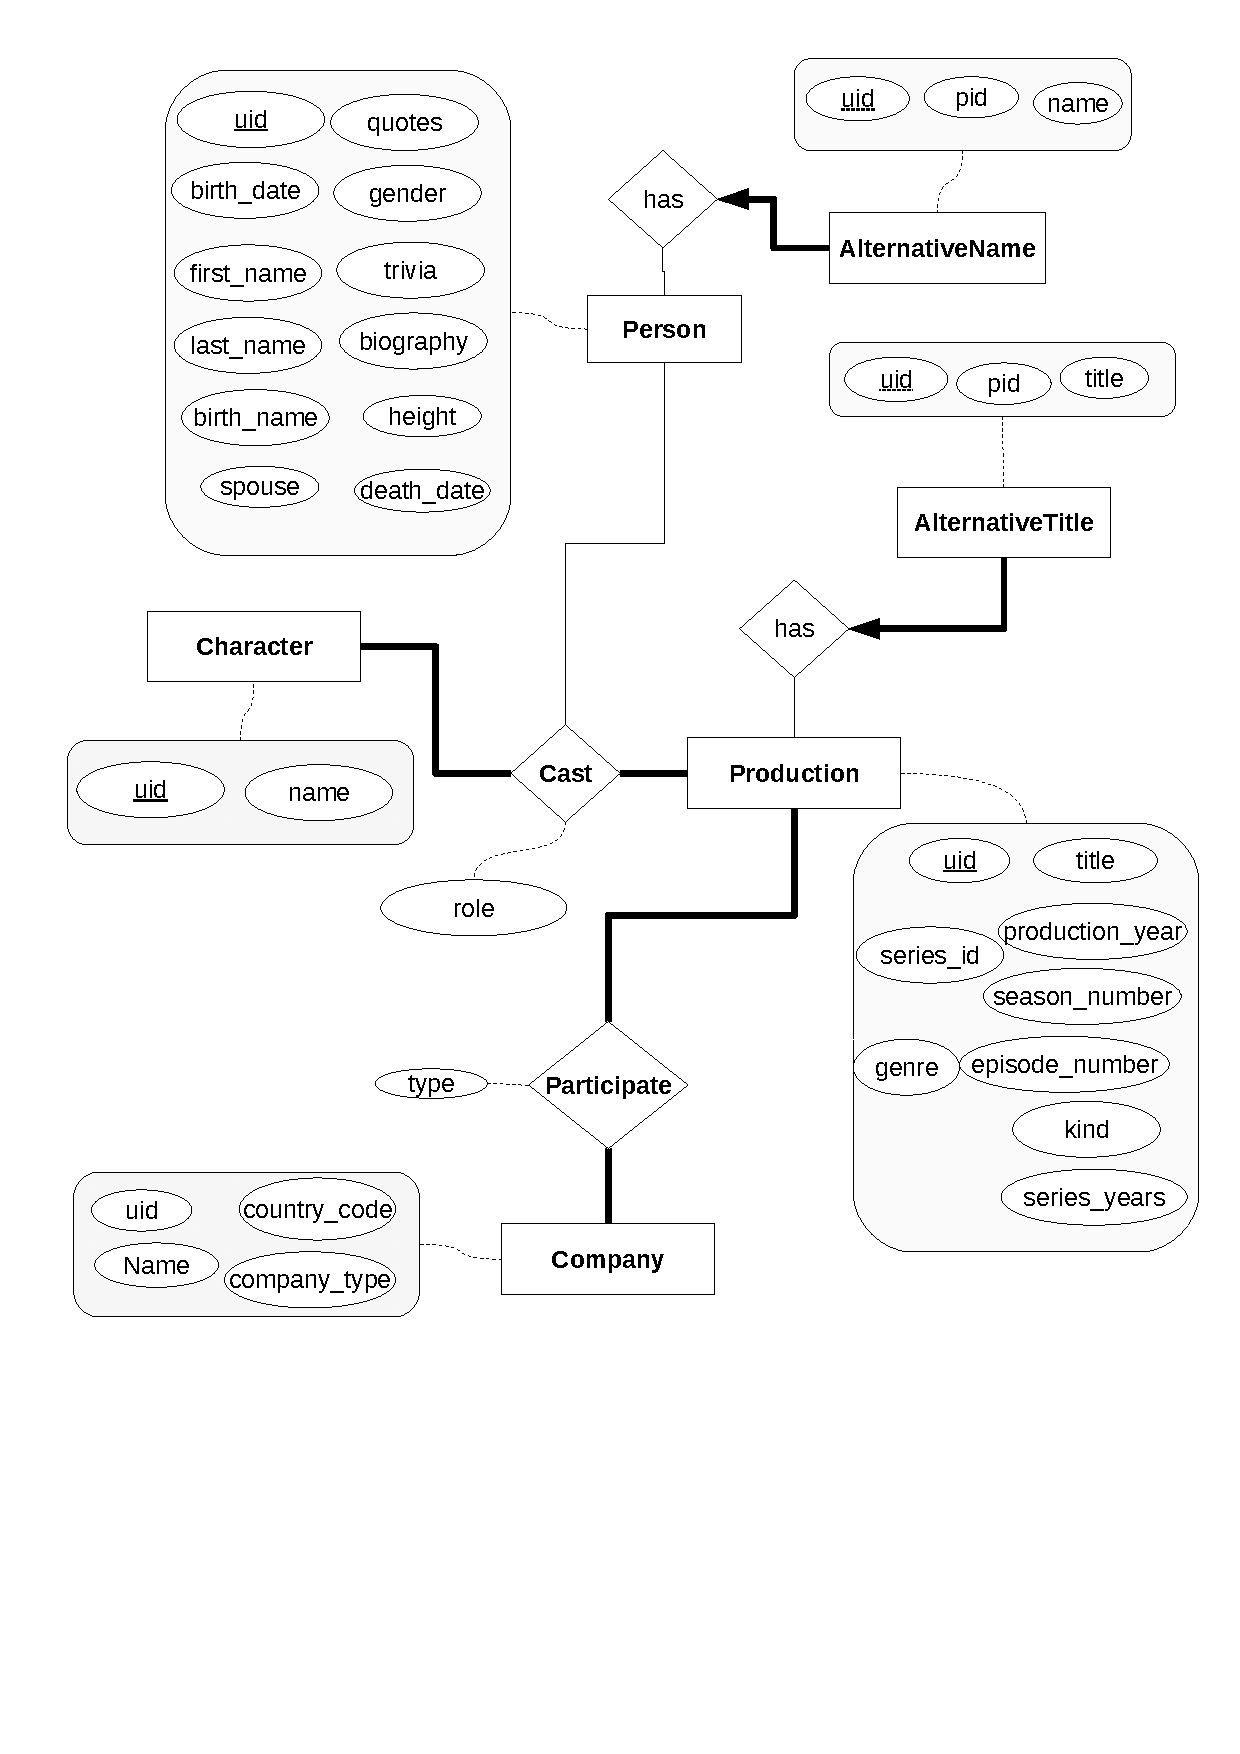
\includepdf[pages={1}]{Diagrame_ER.pdf}

\section{Table creation}
We will implement the next deliverables using our own server with PostGreSQL.
As such the types used in the following CREATE TABLE possibly doesn't work well in an
Oracle DB environnement.
\begin{lstlisting}[
           language=SQL,
           showspaces=false,
           basicstyle=\ttfamily,
           numbers=left,
           numberstyle=\tiny,
           commentstyle=\color{gray}
        ]
CREATE TABLE Person
   (uid INTEGER NOT NULL,
    first_name CHAR(75) NOT NULL,
    last_name CHAR(75) NOT NULL,
    gender CHAR(1),
    trivia TEXT,
    quotes VARCHAR(4000),
    birth DATE,
    death DATE,
    biography TEXT,
    spouse CHAR(100),
    height DOUBLE PRECISION,
    primary key (uid));

CREATE TABLE AlternativeName
   (uid INTEGER NOT NULL,
    pid INTEGER NOT NULL,
    name CHAR(60) NOT NULL,
    primary key (uid)
    foreign key (pid) references Person(uid),
    ON DELETE CASCADE);

CREATE TABLE Character
   (uid INTEGER NOT NULL,
    name CHAR(60) NOT NULL,
    primary key (uid),
    );

CREATE TABLE Cast
   (cid INTEGER,
    perid INTEGER NOT NULL,
    prodid INTEGER NOT NULL,
    rid SMALLINT NOT NULL,
    primary key (cid, perid, prodid, role),
    foreign key (cid) references Character (uid),
    foreign key (perid) references Person (uid),
    foreign key (prodid) references Production (uid)
    foreign key (rid) references Role (uid));

CREATE TABLE Role
   (uid SMALLINT NOT NULL,
    title CHAR(20) NOT NULL,
    primary key (uid));

CREATE TABLE Production
   (uid INTEGER NOT NULL,
    title CHAR(80) NOT NULL,
    currency CHAR(3),
    budget INTEGER,
    primary key (uid));

CREATE TABLE Participate
   (pid INTEGER NOT NULL,
    cid INTEGER NOT NULL,
    type CHAR(20) NOT NULL,
    primary key (pid, cid)
    foreign key (pid) references Production(uid),
    foreign key (cid) references Company(uid));

CREATE TABLE Company
   (uid INTEGER NOT NULL,
    name CHAR(20) NOT NULL,
    country_code CHAR(6),
    primary key (uid));

CREATE TABLE AlternativeTitle
   (uid INTEGER NOT NULL,
    pid INTEGER,
    title CHAR (30),
    primary key (uid, pid)
    foreign key (pid) references Production (uid),
    ON DELETE CASCADE);
\end{lstlisting}


\section{Discussion about constraint}
A person can have one or more alternative name but an alternative name can describe only one person. We thus have a one-to-many relationship set. Also if the person is deleted from the database, his alternative names (if any) will be too. We thus created a weak entity for alternative name. \\

Same thing for the production that can have one or more alternative title, we created a weak entity for alternative title. \\

A production cast make the connection between the production, the person and the character (if any). We thus made a ternary relationship between the three entity person, character and production. We add the role of the person as an attribute of the relationship set. A character exist only if related to at least one person and one production. The person and production entity don't have this constraint since a production can have only a director that won't have any character.  \\

Companies can be involved into production. They can play roles of different type (for example production, distribution), thus we added an attribute to the relationship "participate" called type (since the data description was changed in that way before the deadline this justification isn't relevant any more). A production need to have at least one company involved.  \\
 

\end{document}
